\documentclass[11pt,a4paper]{article}

% ==============================================================================
% PACKAGES & MINIMALIST SYSTEM CONFIGURATION
% ==============================================================================
\usepackage[utf8]{inputenc}
\usepackage[T1]{fontenc}
\usepackage{lmodern}
\usepackage[margin=0.9in,headheight=14pt]{geometry}
\usepackage{microtype}
\usepackage{amsmath,amssymb}
\usepackage{booktabs}
\usepackage{tabularx}
\usepackage{array}
\usepackage{float}
\usepackage{enumitem}
\usepackage{xcolor}
\usepackage{tikz}
\usetikzlibrary{shapes.geometric,arrows.meta,positioning,calc}
\usepackage{fancyhdr}
\usepackage{titlesec}

% Hyperref setup
\usepackage[
    colorlinks=true,
    linkcolor=midnightblue,
    citecolor=teal,
    urlcolor=primary,
    bookmarks=true,
    bookmarksnumbered=true,
    pdfauthor={Abu Zafor, Anamul Haque},
    pdftitle={UniExpert - Software Requirements Specification (Minimal Edition)},
    pdfsubject={SE 331 Software Engineering Design Capstone Project},
    pdfkeywords={SRS, Requirements Engineering, IEEE 830, UniExpert, AI Matchmaking, Fall 2026}
]{hyperref}

% Academic Minimalist Color Palette
\definecolor{primary}{RGB}{20, 50, 95}       % Deep Academic Navy
\definecolor{secondary}{RGB}{40, 110, 180}   % Muted Steel Blue
\definecolor{darkslate}{RGB}{35, 45, 55}     % Dark Neutral Gray
\definecolor{midnightblue}{RGB}{15, 35, 75}  % Header Blue
\definecolor{lightbg}{RGB}{248, 250, 252}    % Soft Off-White

% Section Heading Formatting (Minimalist Underlined Style)
\titleformat{\section}
  {\normalfont\large\bfseries\color{primary}}{\thesection}{0.8em}{}[\titlerule]
\titleformat{\subsection}
  {\normalfont\normalsize\bfseries\color{secondary}}{\thesubsection}{0.8em}{}
\titleformat{\subsubsection}
  {\normalfont\small\bfseries\color{darkslate}}{\thesubsubsection}{0.8em}{}

\titlespacing*{\section}{0pt}{1.2ex plus 0.3ex minus 0.2ex}{0.6ex plus 0.2ex}
\titlespacing*{\subsection}{0pt}{1.0ex plus 0.2ex minus 0.2ex}{0.4ex}

% Header and Footer
\pagestyle{fancy}
\fancyhf{}
\fancyhead[L]{\small\color{gray}\textbf{UniExpert} $|$ Software Requirements Specification (Minimal Edition)}
\fancyhead[R]{\small\color{gray}SE 331 $\cdot$ Fall 2026}
\fancyfoot[L]{\small\color{gray}Department of Software Engineering}
\fancyfoot[R]{\small\color{gray}\thepage}
\renewcommand{\headrulewidth}{0.4pt}
\renewcommand{\footrulewidth}{0.4pt}

% ==============================================================================
% DOCUMENT BEGINS
% ==============================================================================
\begin{document}

% ------------------------------------------------------------------------------
% MINIMAL COVER PAGE
% ------------------------------------------------------------------------------
\begin{titlepage}
    \centering
    \vspace*{1.2cm}
    
    {\large\scshape Department of Software Engineering}\\[0.2cm]
    {\normalsize Faculty of Science \& Information Technology}\\[2.2cm]
    
    {\Huge\bfseries\color{primary} UniExpert}\\[0.45cm]
    {\LARGE\bfseries\color{darkslate} AI-Powered Expert Discovery and Academic Collaboration Platform}\\[0.75cm]
    {\large\color{secondary} Software Requirements Specification (SRS) --- Minimal Edition}\\[0.2cm]
    {\small\textit{Conforming to IEEE Std 830-1998 / ISO/IEC/IEEE 29148:2018 Engineering Standard}}\\[0.4cm]
    \rule{3.2in}{0.5pt}\\[0.55cm]
    
    {\normalsize\textbf{Course:} SE 331 --- Software Engineering Design Capstone Project}\\[0.22cm]
    {\normalsize\textbf{Semester:} Fall 2026 \quad $\cdot$ \quad \textbf{Duration:} October -- December 2026}\\[3.0cm]
    
    \begin{minipage}[t]{0.48\textwidth}
        \begin{flushleft}
            {\small\scshape Prepared By (Student Team)}\\[0.35cm]
            \textbf{Abu Zafor}\\
            {\small Student ID: 232-35-331}\\[0.25cm]
            \textbf{Anamul Haque}\\
            {\small Student ID: 232-35-285}
        \end{flushleft}
    \end{minipage}
    \hfill
    \begin{minipage}[t]{0.45\textwidth}
        \begin{flushright}
            {\small\scshape Supervised By}\\[0.35cm]
            \textbf{Mr. Md. Shohel Arman}\\[0.12cm]
            {\small Assistant Professor}\\
            {\small Department of Software Engineering}
        \end{flushright}
    \end{minipage}
    
    \vfill
    
    {\small\textbf{Date of Submission:} October 14, 2026}
    \vspace*{0.8cm}
\end{titlepage}

\thispagestyle{plain}

% ------------------------------------------------------------------------------
% 1. DOCUMENT CONTROL & EXECUTIVE BASELINE
% ------------------------------------------------------------------------------
\section{Document Control and Specification Baseline}

This minimalist Software Requirements Specification (SRS) establishes the binding technical, functional, and non-functional requirements for \textbf{UniExpert} under course \textbf{SE 331 (Software Engineering Design Capstone Project)} for Fall 2026.

\begin{table}[H]
\centering
\small
\begin{tabularx}{\textwidth}{@{}l l l X l@{}}
\toprule
\textbf{Ver.} & \textbf{Date} & \textbf{Author(s)} & \textbf{Scope and Summary of Major Changes} & \textbf{Status} \\
\midrule
0.1 & Oct 02, 2026 & A. Zafor, A. Haque & Initial requirements elicitation, actor profiles, and scope drafting. & Draft \\
0.5 & Oct 08, 2026 & A. Zafor, A. Haque & Complete IEEE 830 functional modules and scoring algorithm definitions. & Reviewed \\
1.0 & Oct 14, 2026 & A. Zafor, A. Haque & Minimalist Baseline SRS compiled for Capstone Committee approval. & Approved \\
\bottomrule
\end{tabularx}
\caption{Document Revision Control}
\label{tab:doc_control}
\end{table}

\vspace{-0.2cm}
\subsection{Executive Overview and IEEE 830 Conventions}
UniExpert transforms academic discovery from rigid keyword lookups into an intelligent, problem-first matching workflow. Students describe research goals in natural language; the system extracts semantic skill entities, indexes candidate profiles in vector stores, executes multi-criteria ranking, and manages collaboration through an auditable Finite State Machine (FSM).
\begin{itemize}[leftmargin=*,noitemsep]
    \item \textbf{Requirement Notation:} Functional requirements are identified as \texttt{FR-[Module]-[Num]}. Non-functional requirements are identified as \texttt{NFR-[Category]-[Num]}.
    \item \textbf{MoSCoW Prioritization:} \textbf{[M]} Must-Have (mandatory MVP scope); \textbf{[S]} Should-Have (high-priority evaluation feature); \textbf{[C]} Could-Have (desirable extension); \textbf{[W]} Won't-Have (deferred out-of-scope).
    \item \textbf{Normative Compliance:} RFC 2119 keywords (\textbf{SHALL}, \textbf{SHOULD}, \textbf{MAY}) define requirement binding.
\end{itemize}

\begin{table}[H]
\centering
\small
\begin{tabularx}{\textwidth}{@{}l p{4.0cm} X@{}}
\toprule
\textbf{Acronym} & \textbf{Full Term} & \textbf{Operational Definition in UniExpert} \\
\midrule
\textbf{EFS} & Expert Finding System & Information retrieval system identifying experts based on domain competencies. \\
\textbf{HNSW} & Hierarchical Navigable Small World & Graph-based vector indexing algorithm in Qdrant for approximate nearest neighbors. \\
\textbf{XAI} & Explainable Artificial Intelligence & Justification subsystem articulating human-readable match rationales. \\
\textbf{FSM} & Finite State Machine & Formal state transition model enforcing valid collaboration proposal lifecycles. \\
\textbf{RBAC} & Role-Based Access Control & Security model segmenting permissions across students, experts, and admins. \\
\textbf{NDCG} & Norm. Discounted Cumulative Gain & Standard information retrieval metric evaluating graded ranking relevance. \\
\bottomrule
\end{tabularx}
\caption{Glossary of Operational Acronyms}
\label{tab:glossary}
\end{table}

\clearpage
% ------------------------------------------------------------------------------
% 2. OVERALL DESCRIPTION & ARCHITECTURAL CONTEXT
% ------------------------------------------------------------------------------
\section{Overall Description and System Context}

\subsection{System Context Diagram}
UniExpert is a decoupled web application interfacing with institutional users, academic bibliometric registries, and vector search engines. Figure~\ref{fig:srs_context} illustrates system boundaries and external interfaces.

\begin{figure}[H]
\centering
\resizebox{0.90\linewidth}{!}{%
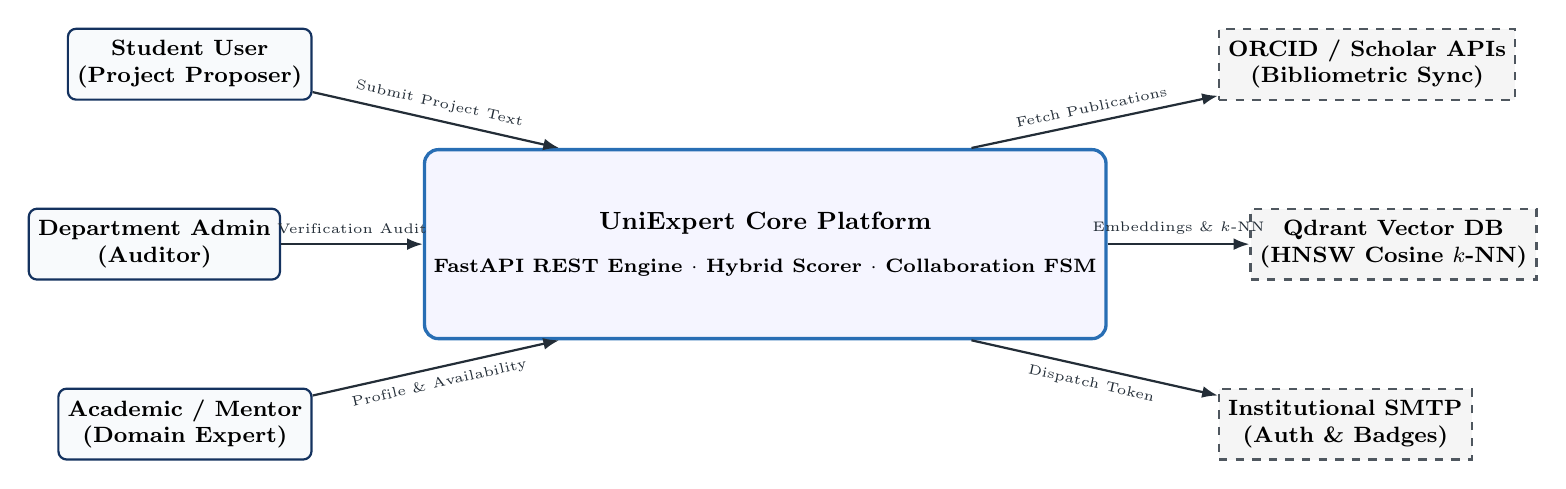
\begin{tikzpicture}[
    actor/.style={rectangle, draw=primary, fill=lightbg, rounded corners=3pt, thick, align=center, font=\footnotesize\bfseries, minimum height=0.9cm, minimum width=2.5cm},
    core/.style={rectangle, draw=secondary, fill=blue!4, rounded corners=5pt, line width=1.2pt, align=center, font=\small\bfseries, minimum height=2.4cm, minimum width=5.6cm},
    ext/.style={rectangle, draw=darkslate!80, fill=gray!8, dashed, thick, align=center, font=\footnotesize\bfseries, minimum height=0.9cm, minimum width=2.5cm},
    flow/.style={-{Latex[length=2.0mm]}, thick, color=darkslate}
]
    % Core
    \node[core] (sys) {\textbf{UniExpert Core Platform}\\[0.15cm]\scriptsize FastAPI REST Engine $\cdot$ Hybrid Scorer $\cdot$ Collaboration FSM};

    % Actors
    \node[actor, above left=0.6cm and 1.4cm of sys] (student) {Student User\\(Project Proposer)};
    \node[actor, below left=0.6cm and 1.4cm of sys] (expert) {Academic / Mentor\\(Domain Expert)};
    \node[actor, left=1.8cm of sys] (admin) {Department Admin\\(Auditor)};

    % External Systems
    \node[ext, above right=0.6cm and 1.4cm of sys] (orcid) {ORCID / Scholar APIs\\(Bibliometric Sync)};
    \node[ext, below right=0.6cm and 1.4cm of sys] (smtp) {Institutional SMTP\\(Auth \& Badges)};
    \node[ext, right=1.8cm of sys] (qdrant) {Qdrant Vector DB\\(HNSW Cosine $k$-NN)};

    % Flows
    \draw[flow] (student) -- node[above,sloped,font=\tiny] {Submit Project Text} (sys.155);
    \draw[flow] (expert) -- node[below,sloped,font=\tiny] {Profile \& Availability} (sys.205);
    \draw[flow] (admin) -- node[above,font=\tiny] {Verification Audit} (sys.west);
    
    \draw[flow] (sys.25) -- node[above,sloped,font=\tiny] {Fetch Publications} (orcid);
    \draw[flow] (sys.335) -- node[below,sloped,font=\tiny] {Dispatch Token} (smtp);
    \draw[flow] (sys.east) -- node[above,font=\tiny] {Embeddings \& $k$-NN} (qdrant);
\end{tikzpicture}%
}
\caption{UniExpert System Context and External Interface Model}
\label{fig:srs_context}
\end{figure}

\subsection{User Classes and Operational Privileges}
\begin{table}[H]
\centering
\small
\begin{tabularx}{\textwidth}{@{}l p{3.2cm} X l@{}}
\toprule
\textbf{User Role} & \textbf{Authentication Basis} & \textbf{System Capabilities and Operational Permissions} & \textbf{Activity} \\
\midrule
\textbf{Student} & Verified university email & Submits proposals, inspects matches, forms teams, dispatches collaboration requests. & Daily / Weekly \\
\textbf{Expert (Faculty)} & Tier 1--3 verified badge & Publishes research skills, configures blackout calendars, accepts/declines requests. & Weekly \\
\textbf{Industry Mentor} & Tier 4 corporate badge & Reviews applied capstones, provides industry mentoring within set capacity. & Bi-weekly \\
\textbf{Administrator} & Multi-factor admin account & Approves verification documentation, reviews audit trails, inspects telemetry. & Periodic \\
\bottomrule
\end{tabularx}
\caption{User Classes and Operational Profiles}
\label{tab:user_profiles}
\end{table}

\subsection{Design Constraints and Operating Environment}
\begin{itemize}[leftmargin=*,noitemsep]
    \item \textbf{Hosting \& Runtime:} Linux server (Ubuntu 22.04 LTS), Python 3.11+ ASGI (FastAPI), React 18+ Web Client, PostgreSQL 16 relational DB, Qdrant 1.8+ vector DB, Redis 7.2 cache.
    \item \textbf{Inference Optimization:} Zero-shot NLP extraction and dense embeddings (\texttt{all-MiniLM-L6-v2}) must run on multi-core CPU architectures via ONNX Runtime without mandatory cloud GPU dependencies.
    \item \textbf{Compliance:} Student proposals and private communications protected by TLS 1.3 in transit and AES-256 at rest, respecting institutional FERPA privacy mandates.
\end{itemize}

\clearpage
% ------------------------------------------------------------------------------
% 3. CONSOLIDATED FUNCTIONAL REQUIREMENTS MATRIX (PART I)
% ------------------------------------------------------------------------------
\section{Consolidated Functional Requirements Matrix}

To maintain high information density, the 20 functional requirements covering all 7 core modules are partitioned into two structured engineering matrices: Table~\ref{tab:fr_matrix_1} (Core Discovery Modules 1 to 4) and Table~\ref{tab:fr_matrix_2} (Advanced Collaboration Modules 5 to 7).

\begin{table}[H]
\centering
\footnotesize
\begin{tabularx}{\textwidth}{@{}l l c X@{}}
\toprule
\textbf{Req ID} & \textbf{Feature / Subsystem} & \textbf{Pri.} & \textbf{Normative Functional Specification} \\
\midrule
\multicolumn{4}{@{}l}{\textbf{Module 1: Authentication and Identity Management}} \\
\texttt{FR-AUTH-01} & Registration \& Activation & \textbf{[M]} & The system SHALL allow students and mentors to register unique accounts. Institutional email domains (\texttt{.edu}) SHALL trigger automated HMAC activation tokens (24h TTL). \\
\texttt{FR-AUTH-02} & RBAC \& Session Tokens & \textbf{[M]} & The system SHALL enforce strict RBAC across \texttt{STUDENT}, \texttt{EXPERT}, and \texttt{ADMIN}. Sessions SHALL use Ed25519-signed JWTs (15m access, 7d HTTP-only refresh). \\
\midrule
\multicolumn{4}{@{}l}{\textbf{Module 2: Profile Engineering and Taxonomy Management}} \\
\texttt{FR-PROF-03} & Student Academic Profile & \textbf{[M]} & The system SHALL maintain student profiles recording department, degree program, research interests, past projects, and CV attachments (PDF, max 5MB). \\
\texttt{FR-PROF-04} & Multi-Tier Credential Badging & \textbf{[M]} & The system SHALL enforce a 4-tier verification scheme: Tier 1 (Institutional Email), Tier 2 (ORCID Sync with $\ge 2$ papers), Tier 3 (Admin Appointment Audit), Tier 4 (Corporate Domain). \\
\texttt{FR-PROF-05} & Structured Skill Taxonomy & \textbf{[M]} & The system SHALL maintain a hierarchical academic skill ontology across engineering, AI, agriculture, and business with automated synonym aliasing (e.g., ``CV'' $\rightarrow$ ``Computer Vision''). \\
\midrule
\multicolumn{4}{@{}l}{\textbf{Module 3: Natural Language Problem Ingestion and NLP Extraction}} \\
\texttt{FR-NLP-06} & Unstructured Problem Ingestion & \textbf{[M]} & The system SHALL accept freeform student research statements (50--2,000 words), project title, expected methodology, and target semester timelines. \\
\texttt{FR-NLP-07} & Zero-Shot Entity Extraction & \textbf{[M]} & The system SHALL extract domain classifications, technical skill prerequisites, and methodological paradigms using zero-shot classification with confidence scores $\ge 0.60$. \\
\texttt{FR-NLP-08} & Interactive Tag Refinement & \textbf{[S]} & The system SHALL provide students with an interactive tag manager to adjust weights, prune spurious keywords, and insert custom required competencies prior to search. \\
\midrule
\multicolumn{4}{@{}l}{\textbf{Module 4: Semantic Matching and Hybrid Recommendation Engine}} \\
\texttt{FR-REC-09} & Vector Embedding Generation & \textbf{[M]} & The system SHALL project project texts and expert profiles into 384-dimensional dense vectors using \texttt{all-MiniLM-L6-v2} indexed in Qdrant with HNSW graphs ($M=16$). \\
\texttt{FR-REC-10} & Multi-Criteria Hybrid Scoring & \textbf{[M]} & The system SHALL rank experts using composite score $\mathcal{S}(u, e) = \sum_{i=1}^5 w_i C_i$ (Eq.~\ref{eq:srs_match}), combining semantic similarity, skill overlap, bibliometrics, tier, and availability. \\
\texttt{FR-REC-11} & Explainable AI (XAI) Justifications & \textbf{[M]} & The system SHALL generate human-readable explanations detailing skill intersection counts, relevant publications, and availability rationales for every recommendation. \\
\texttt{FR-REC-12} & Faceted Filtering \& Re-Ranking & \textbf{[M]} & The system SHALL permit dynamic client-side filtering by verification tier, affiliation, and availability status without requiring re-computation of dense embeddings. \\
\bottomrule
\end{tabularx}
\caption{Functional Requirements Matrix --- Modules 1 to 4 (Authentication, Profiles, NLP, Matching)}
\label{tab:fr_matrix_1}
\end{table}

\clearpage
% ------------------------------------------------------------------------------
% 3. CONSOLIDATED FUNCTIONAL REQUIREMENTS MATRIX (PART II) & FORMULATIONS
% ------------------------------------------------------------------------------
\begin{table}[H]
\centering
\footnotesize
\begin{tabularx}{\textwidth}{@{}l l c X@{}}
\toprule
\textbf{Req ID} & \textbf{Feature / Subsystem} & \textbf{Pri.} & \textbf{Normative Functional Specification} \\
\midrule
\multicolumn{4}{@{}l}{\textbf{Module 5: Multidisciplinary Team Formation and Gap Analysis}} \\
\texttt{FR-TEAM-13} & Project Domain Decomposition & \textbf{[S]} & The system SHALL automatically decompose interdisciplinary projects into discrete sub-domains (e.g., Computer Vision and Pathology) generating parallel search tracks. \\
\texttt{FR-TEAM-14} & Set-Cover Skill Gap Detection & \textbf{[S]} & Given accepted advisory members $\mathcal{M}$, the system SHALL compute unresolved gaps $\Delta \mathcal{K} = \mathcal{K}_u \setminus \bigcup_{e \in \mathcal{M}} \mathcal{K}_e$ (Eq.~\ref{eq:srs_gap}) and recommend complementary recruits. \\
\texttt{FR-TEAM-15} & Side-by-Side Comparison Matrix & \textbf{[S]} & The system SHALL render comparative evaluations for up to 3 candidate experts comparing publications, badge tiers, skill overlap percentages, and active advising load. \\
\midrule
\multicolumn{4}{@{}l}{\textbf{Module 6: Collaboration Lifecycle and Workspace Management}} \\
\texttt{FR-COL-16} & Formal Collaboration FSM & \textbf{[M]} & The system SHALL enforce an auditable FSM (\texttt{SUBMITTED} $\rightarrow$ \texttt{UNDER\_REVIEW} $\rightarrow$ \texttt{ACCEPTED} / \texttt{DECLINED} $\rightarrow$ \texttt{ACTIVE} $\rightarrow$ \texttt{COMPLETED}). Illegal transitions SHALL return HTTP 409. \\
\texttt{FR-COL-17} & Anti-Fatigue Quotas \& Blackouts & \textbf{[M]} & The system SHALL enforce a monthly incoming quota (max 5 active requests per faculty), blackout calendar toggles, and 14-day auto-expiration on unanswered requests. \\
\texttt{FR-COL-18} & Shared Workspace \& Messaging & \textbf{[M]} & Upon reaching \texttt{ACCEPTED}, the system SHALL spin up a shared workspace featuring milestone checklists, file exchange (PDF/ZIP, max 10MB), and audit-logged messaging. \\
\midrule
\multicolumn{4}{@{}l}{\textbf{Module 7: Governance, Feedback, and Administration}} \\
\texttt{FR-GOV-19} & Double-Blind Peer Review & \textbf{[S]} & Upon project completion, both student and mentor SHALL submit mutual 4-axis reviews (responsiveness, mentorship, goal attainment, professionalism) updating profile scores. \\
\texttt{FR-GOV-20} & Administrative Audit Portal & \textbf{[M]} & The system SHALL provide departmental admins with a verification queue, document inspector, user dispute resolution console, and system telemetry dashboard. \\
\bottomrule
\end{tabularx}
\caption{Functional Requirements Matrix --- Modules 5 to 7 (Teams, Lifecycle, Governance)}
\label{tab:fr_matrix_2}
\end{table}

\vspace{-0.2cm}
\subsection{Mathematical Formulations of Core Engines}
\noindent\textbf{(1) Hybrid Recommendation Formulation (FR-REC-10):}
\begin{equation}
    \label{eq:srs_match}
    \mathcal{S}(u, e) = w_1 \cdot \mathcal{D}(u, e) + w_2 \cdot \mathcal{K}(u, e) + w_3 \cdot \mathcal{R}(u, e) + w_4 \cdot \mathcal{V}(e) + w_5 \cdot \mathcal{A}(u, e)
\end{equation}
where $\mathcal{D}(u, e) = \frac{\vec{v}_u \cdot \vec{v}_e}{\|\vec{v}_u\|\|\vec{v}_e\|}$ is dense semantic cosine similarity, $\mathcal{K}(u, e) = \frac{|\mathcal{K}_u \cap \mathcal{K}_e|}{|\mathcal{K}_u|}$ is weighted skill overlap, $\mathcal{R}(u, e)$ is normalized citation/publication count, $\mathcal{V}(e) \in \{0.25, 0.50, 0.75, 1.0\}$ represents verification tier authority, and $\mathcal{A}(u, e) = 1 - \frac{\text{ActiveLoad}}{\text{MaxLoad}}$ is availability capacity. Baseline weights: $w_1=0.30, w_2=0.25, w_3=0.20, w_4=0.15, w_5=0.10$ ($\sum w_i = 1.0$).

\vspace{0.2cm}
\noindent\textbf{(2) Advisory Skill Gap Detection (FR-TEAM-14):}
\begin{equation}
    \label{eq:srs_gap}
    \Delta \mathcal{K} = \mathcal{K}_u \setminus \bigcup_{e \in \mathcal{M}} \mathcal{K}_e, \qquad \text{where } \mathcal{M} = \{e_1, e_2, \dots, e_m\}
\end{equation}
When $|\Delta \mathcal{K}| > 0$, the system executes a greedy set-cover selection to nominate candidate experts $e^* = \arg\max_{e \notin \mathcal{M}} |\mathcal{K}_e \cap \Delta \mathcal{K}|$.

\clearpage
% ------------------------------------------------------------------------------
% 4. NON-FUNCTIONAL REQUIREMENTS & DATA REQUIREMENTS
% ------------------------------------------------------------------------------
\section{Non-Functional Requirements and Industrial Benchmarks}

\begin{table}[H]
\centering
\small
\begin{tabularx}{\textwidth}{@{}l p{3.2cm} X l@{}}
\toprule
\textbf{Req ID} & \textbf{Category / Metric} & \textbf{Technical Specification \& Acceptance Threshold} & \textbf{Verification} \\
\midrule
\texttt{NFR-PERF-01} & Search Response Latency & $P_{95}$ semantic retrieval latency SHALL be $\le 250\text{ ms}$ over 10,000 indexed profiles. & k6 Load Test \\
\texttt{NFR-PERF-02} & NLP Extraction Speed & Entity extraction for a 500-word statement SHALL finish within $\le 1.2\text{ s}$ on multi-core CPU. & Benchmark \\
\texttt{NFR-PERF-03} & System Concurrency & API server SHALL sustain 200 concurrent requests with error rate $\le 0.1\%$. & Stress Test \\
\texttt{NFR-PERF-04} & Frontend First Render & Web client First Contentful Paint (FCP) SHALL be $< 1.0\text{ s}$ over standard 4G broadband. & Lighthouse \\
\midrule
\texttt{NFR-SEC-01}  & Data in Transit & All communications SHALL be encrypted under TLS 1.3 with strict HSTS enforcement. & SSL Labs (A+) \\
\texttt{NFR-SEC-02}  & Password Security & Passwords salted and hashed with Argon2id ($m=64\text{MB}, t=3, p=4$); plaintext never logged. & Code Audit \\
\texttt{NFR-SEC-03}  & Session Protection & JWTs signed with asymmetric keys; refresh tokens stored in \texttt{HttpOnly, SameSite=Strict} cookies. & Security Test \\
\texttt{NFR-SEC-04}  & Rate Limiting & Authentication endpoints throttled to 5 failed attempts per minute per IP via Redis. & Penetration Test \\
\midrule
\texttt{NFR-REL-01}  & System Availability & Discovery service SHALL guarantee $\ge 99.9\%$ monthly uptime (excluding scheduled windows). & Uptime Monitor \\
\texttt{NFR-REL-02}  & Backup \& Recovery & Daily automated PostgreSQL WAL archiving achieving RPO $\le 1\text{ hour}$ and RTO $\le 30\text{ minutes}$. & Disaster Drill \\
\texttt{NFR-REL-03}  & Fallback Degradation & If Qdrant is temporarily offline, system SHALL gracefully degrade to PostgreSQL BM25 keyword search. & Chaos Test \\
\midrule
\texttt{NFR-USE-01}  & Accessibility Compliance & Web interfaces SHALL comply with WCAG 2.1 Level AA with complete keyboard/screen-reader support. & axe-core Audit \\
\texttt{NFR-USE-02}  & Usability Evaluation & The platform SHALL achieve a System Usability Scale (SUS) score $\ge 80$ during Capstone UAT. & User Survey \\
\bottomrule
\end{tabularx}
\caption{Non-Functional Requirements and Quality Attributes}
\label{tab:nfr_matrix}
\end{table}

\section{Data Requirements and Relational Data Dictionary}
Relational transactional data resides in PostgreSQL 16 under strict foreign key constraints, while 384-dimensional embeddings are indexed in Qdrant collections.

\begin{table}[H]
\centering
\small
\begin{tabularx}{\textwidth}{@{}l l l X@{}}
\toprule
\textbf{Entity} & \textbf{Attribute Name} & \textbf{Data Type} & \textbf{Constraints and Semantic Purpose} \\
\midrule
\texttt{users} & \texttt{id} & UUID & Primary Key, generated via \texttt{uuid\_generate\_v4()}. \\
& \texttt{email} & VARCHAR(255) & Unique, valid institutional format, B-tree indexed. \\
& \texttt{password\_hash} & VARCHAR(255) & Argon2id cryptographic hash string. \\
& \texttt{role} & ENUM & \texttt{STUDENT}, \texttt{EXPERT}, \texttt{ADMIN}. \\
& \texttt{is\_verified} & BOOLEAN & Default \texttt{FALSE}; set \texttt{TRUE} upon activation token verification. \\
\midrule
\texttt{expert\_profiles} & \texttt{id} & UUID & Primary Key; Foreign Key referencing \texttt{users(id)} on delete cascade. \\
& \texttt{institution} & VARCHAR(255) & University or corporate organization name. \\
& \texttt{verification\_tier} & INTEGER & Values $1, 2, 3, 4$ representing credential authority badge. \\
& \texttt{availability} & ENUM & \texttt{AVAILABLE}, \texttt{LIMITED}, \texttt{BLACKOUT}. \\
& \texttt{max\_load} & INTEGER & Maximum simultaneous active collaborations (default: 3). \\
\midrule
\texttt{projects} & \texttt{id} & UUID & Primary Key. \\
& \texttt{student\_id} & UUID & Foreign Key referencing \texttt{users(id)}. \\
& \texttt{title} & VARCHAR(255) & Project working title. \\
& \texttt{raw\_statement} & TEXT & Natural language problem description (50--2,000 words). \\
& \texttt{embedding\_id} & VARCHAR(64) & Vector UUID reference to Qdrant collection point. \\
\midrule
\texttt{collaborations} & \texttt{id} & UUID & Primary Key. \\
& \texttt{project\_id} & UUID & Foreign Key referencing \texttt{projects(id)}. \\
& \texttt{expert\_id} & UUID & Foreign Key referencing \texttt{expert\_profiles(id)}. \\
& \texttt{state} & ENUM & \texttt{SUBMITTED}, \texttt{ACCEPTED}, \texttt{ACTIVE}, \texttt{COMPLETED}, etc. \\
& \texttt{created\_at} & TIMESTAMPTZ & Immutable UTC timestamp generated at proposal submission. \\
\bottomrule
\end{tabularx}
\caption{Relational Database Data Dictionary}
\label{tab:data_dictionary}
\end{table}

\clearpage
% ------------------------------------------------------------------------------
% 5. REQUIREMENTS TRACEABILITY MATRIX & VERIFICATION PROTOCOL
% ------------------------------------------------------------------------------
\section{Requirements Traceability Matrix (RTM)}

Table~\ref{tab:srs_rtm} links each functional requirement to its responsible architectural subsystem, test case ID, and standard IEEE verification method: \textbf{T} (Test), \textbf{D} (Demonstration), \textbf{A} (Analysis), and \textbf{I} (Inspection).

\begin{table}[H]
\centering
\footnotesize
\begin{tabularx}{\textwidth}{@{}l p{4.6cm} l l c@{}}
\toprule
\textbf{Req ID} & \textbf{Requirement Title} & \textbf{Architectural Module} & \textbf{Test Case ID} & \textbf{Method} \\
\midrule
\texttt{FR-AUTH-01} & Registration \& Token Activation & Auth Service & \texttt{TC-AUTH-01} & T \\
\texttt{FR-AUTH-02} & Role-Based Access Control (RBAC) & Gateway Service & \texttt{TC-AUTH-02} & T \\
\texttt{FR-PROF-03} & Student Profile Management & Profile Service & \texttt{TC-PROF-01} & D \\
\texttt{FR-PROF-04} & Multi-Tier Credential Badging & Verification Service & \texttt{TC-PROF-02} & I, T \\
\texttt{FR-PROF-05} & Academic Skill Taxonomy & Taxonomy Service & \texttt{TC-TAX-01} & T \\
\texttt{FR-NLP-06}  & Project Statement Ingestion & Project Service & \texttt{TC-PROJ-01} & D \\
\texttt{FR-NLP-07}  & Zero-Shot Entity Extraction & AI Inference Engine & \texttt{TC-NLP-01} & A, T \\
\texttt{FR-NLP-08}  & Interactive Tag Refinement & Web Client UI & \texttt{TC-NLP-02} & D \\
\texttt{FR-REC-09}  & Dense Vector Indexing & Qdrant Store Service & \texttt{TC-VEC-01} & T \\
\texttt{FR-REC-10}  & Multi-Criteria Hybrid Ranking & Matchmaking Engine & \texttt{TC-REC-01} & A, T \\
\texttt{FR-REC-11}  & Explainable AI Justifications & XAI Service & \texttt{TC-REC-02} & D, T \\
\texttt{FR-REC-12}  & Dynamic Faceted Filtering & Search Service & \texttt{TC-REC-03} & T \\
\texttt{FR-TEAM-13} & Project Domain Decomposition & Team Service & \texttt{TC-TEAM-01} & A, T \\
\texttt{FR-TEAM-14} & Set-Cover Skill Gap Analysis & Team Service & \texttt{TC-TEAM-02} & A, T \\
\texttt{FR-TEAM-15} & Side-by-Side Comparison Matrix & Web Client UI & \texttt{TC-TEAM-03} & D \\
\texttt{FR-COL-16}  & Collaboration Lifecycle FSM & Collaboration Service & \texttt{TC-COL-01} & T \\
\texttt{FR-COL-17}  & Anti-Fatigue Quotas \& Blackouts & Governance Service & \texttt{TC-COL-02} & T \\
\texttt{FR-COL-18}  & Shared Workspace \& Messaging & Workspace Service & \texttt{TC-COL-03} & D, T \\
\texttt{FR-GOV-19}  & Double-Blind Peer Review & Reputation Service & \texttt{TC-GOV-01} & D \\
\texttt{FR-GOV-20}  & Administrative Audit Dashboard & Admin Service & \texttt{TC-GOV-02} & D, I \\
\bottomrule
\end{tabularx}
\caption{Requirements Traceability Matrix (RTM)}
\label{tab:srs_rtm}
\end{table}

\vspace{-0.1cm}
\section{Verification Strategy and Committee Sign-Off}

\subsection{Testing and Information Retrieval Benchmarking}
\begin{itemize}[leftmargin=*,noitemsep]
    \item \textbf{Continuous Integration (GitHub Actions):} Every commit triggers automated Pytest suites verifying mathematical scoring bounds, FSM state validity, and schema migrations with $\ge 85\%$ line coverage.
    \item \textbf{IR Evaluation Protocol:} Recommendation quality is validated against a 50-query academic benchmark with ground-truth expert relevance judgments evaluating Precision@$K$ ($K=3, 5$) and $NDCG@5$, benchmarked against baseline BM25 lexical search.
    \item \textbf{User Acceptance Testing (UAT):} Scheduled for December 2026 with 20 students and 8 faculty members measuring task completion rate ($\ge 90\%$) and SUS score ($\ge 80$).
\end{itemize}

\vspace{0.4cm}
\subsection{Academic Committee Review and Approval}
The undersigned supervisor and capstone committee members confirm that this Software Requirements Specification (SRS) establishes the agreed baseline for the engineering, evaluation, and grading of \textbf{UniExpert} for the Fall 2026 academic semester.

\vspace{1.0cm}
\noindent
\begin{minipage}[t]{0.48\textwidth}
    \rule{2.8in}{0.5pt}\\[0.2cm]
    \textbf{Mr. Md. Shohel Arman}\\
    Assistant Professor\\
    Department of Software Engineering\\
    Faculty of Science \& Information Technology\\
    \textit{Date:} \rule{1.4in}{0.4pt}
\end{minipage}
\hfill
\begin{minipage}[t]{0.48\textwidth}
    \rule{2.8in}{0.5pt}\\[0.2cm]
    \textbf{Head of Department / Committee Chair}\\
    Department of Software Engineering\\
    Faculty of Science \& Information Technology\\
    \textit{Date:} \rule{1.4in}{0.4pt}
\end{minipage}

\end{document}
